Segundo Leonhardt Euler, o fator mais importante que determina a carga crítica nos elementos comprimidos é a \textbf{esbeltez}. Em função dela, conclui-se que, quanto mais esbelto for o elemento estrutural, menor será sua carga crítica.

A determinação do parâmetro \textbf{esbeltez} ($\lambda$) de um elemento estrutural é função do seu momento de inércia ($I$) de sua seção transversal, que é determinado em função de sua espessura. A propriedade da seção transversal que é usada na determinação da carga crítica é o \textbf{raio de giração da seção transversal} ($i$), que é relativo ao \textbf{momento de inércia}.
\begin{equation}i=\sqrt{\frac{I}{A}}\end{equation}

Onde $i$ é o raio de giração da seção geométrica da peça, sem considerar a presença da armadura; $I$ é o momento de inércia da seção transversal do pilar em relação ao eixo $x$ ou $y$; e $A$ é a área da seção transversal do pilar.

O momento de inércia indica a dificuldade de uma peça girar no eixo escolhido.

Para um pilar em pé em relação à visão em planta:

\begin{figure}[H]
	\begin{center}
	\caption{Exemplo de seção transversal (retangular) para cálculo do momento de inércia.}
    	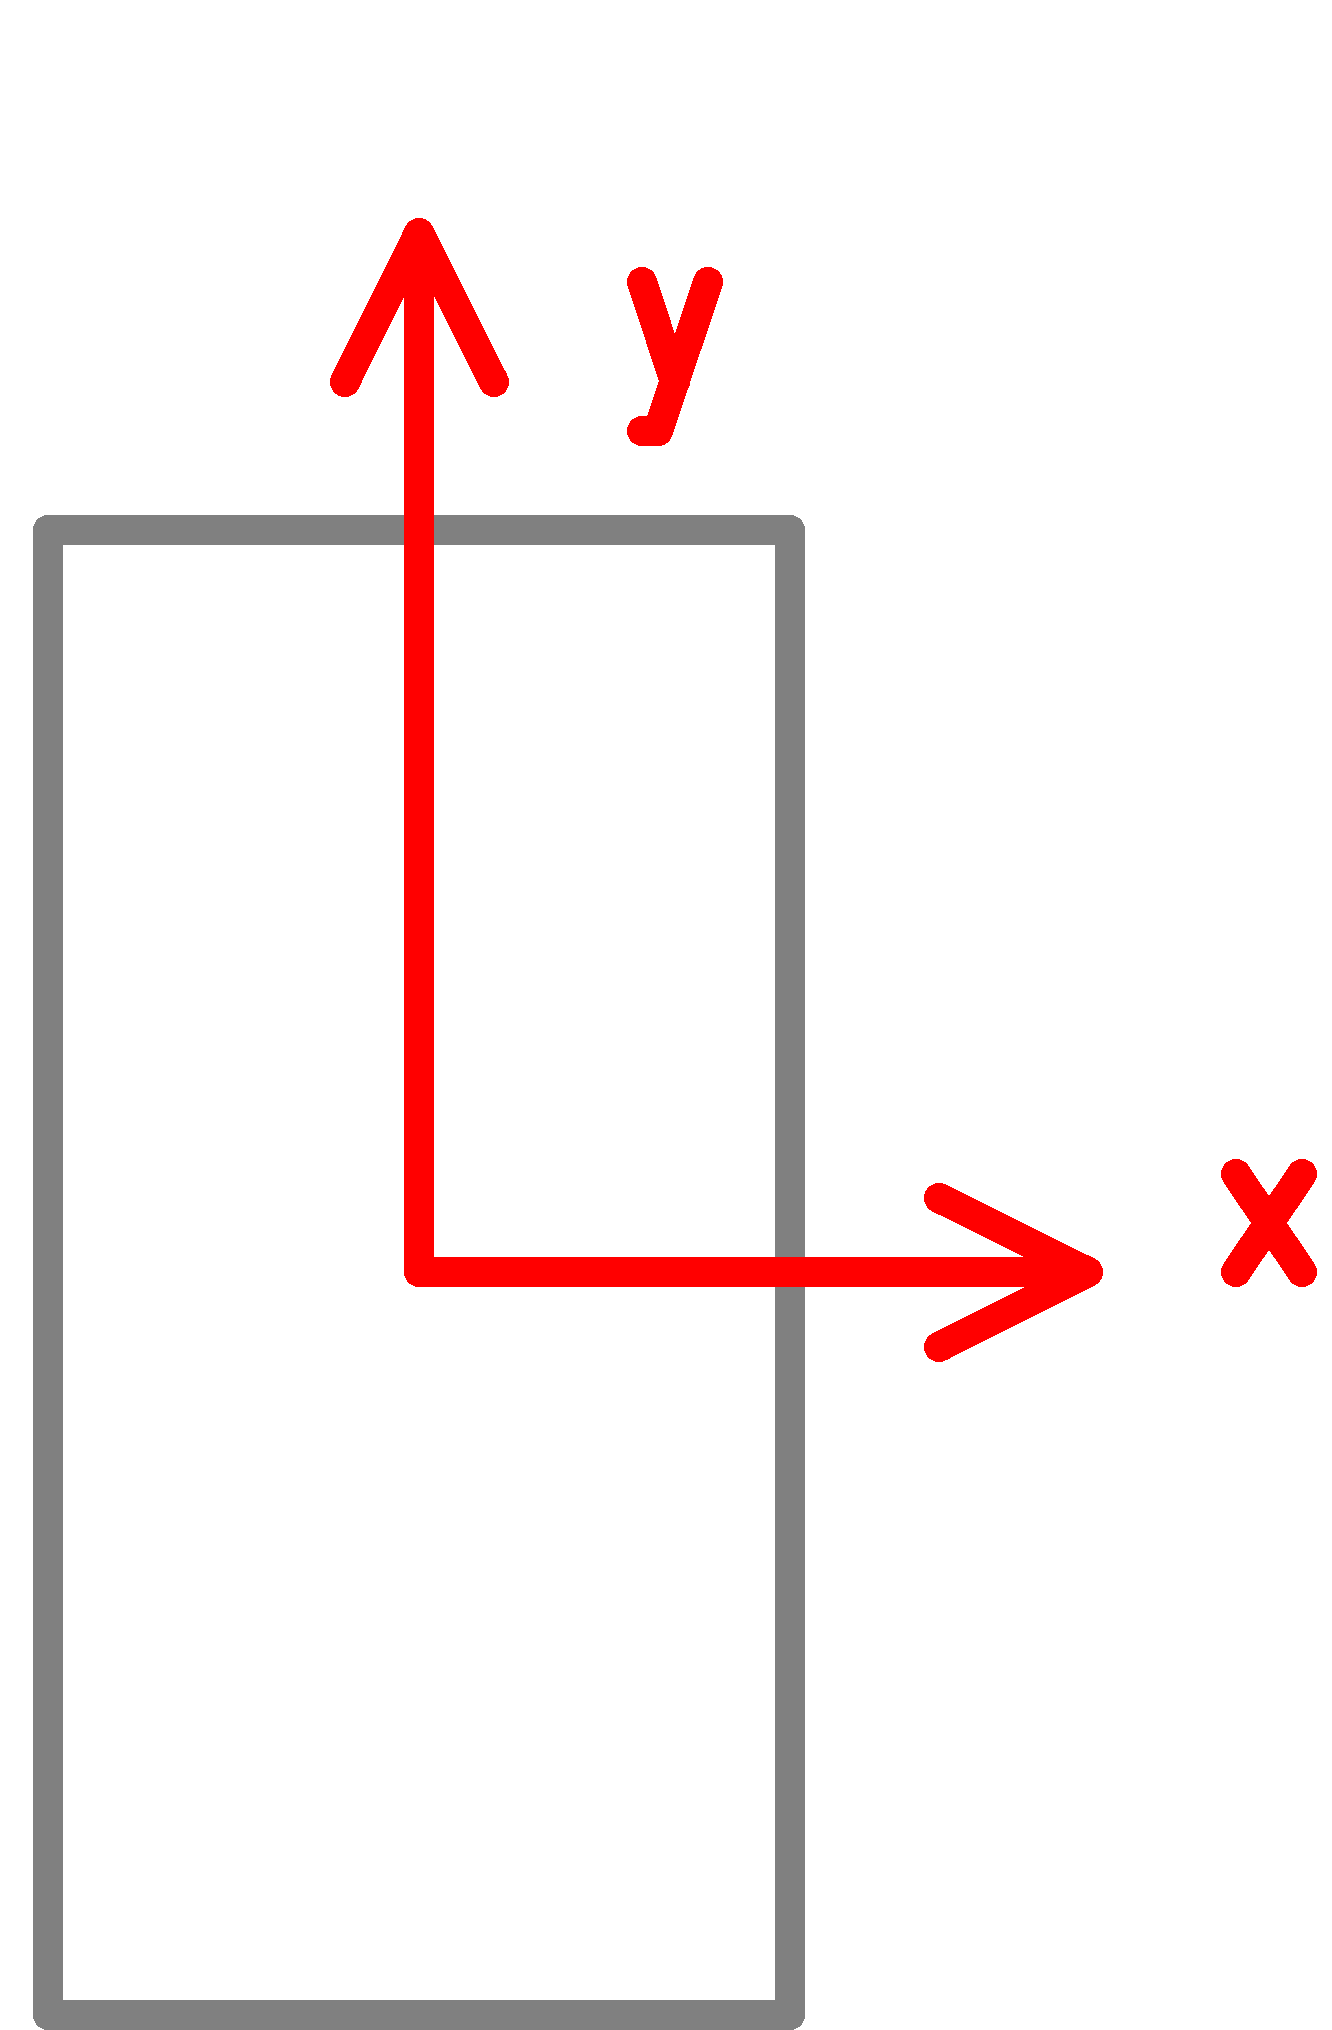
\includegraphics[width=0.1\textwidth]{Indice-de-esbeltez/Imagens/Secao-transversal-pilar.png}
	\end{center}
\end{figure}

Na direção $x$ (a base será sempre a face onde o eixo está olhando). Por exemplo, um pilar $P1$ (20x70):
$$I_x=\frac{b\cdot h^3}{12}=\frac{70\cdot{20}^3}{12}\approx46666,6667\;{cm}^4$$

E na direção $y$:
$$I_y=\frac{b\cdot h^3}{12}=\frac{20\cdot{70}^3}{12}\approx571666,6667\;{cm}^4$$

Ou seja, é muito mais difícil rotacionar no eixo $y$.

O \textbf{Índice de Esbeltez ($\lambda$)} depende do raio de giração e do comprimento de flambagem e possui limites com a finalidade de \textbf{evitar} a grande flexibilidade de peças excessivamente esbeltas.
\begin{equation}\lambda=\frac{L_e}{i}\leqslant200\end{equation}

Para uma seção retangular, o Índice de Esbeltez pode ser definido por:
\begin{equation}\lambda=\frac{\sqrt{12}\cdot L_e}{h}\leqslant200\end{equation}

Já que: \begin{equation}i=\sqrt{\frac{I}{A}}=\sqrt{\frac{\frac{b\cdot h^3}{12}}{b\cdot h}}=\sqrt{\frac{h^2}{12}}=\frac{h}{\sqrt{12}}\end{equation}

A NBR 6118 não admite, em nenhum caso, pilares com $\lambda$ superior a 200 para edificações. O valor de $\lambda$ deve ser calculado tanto na direção $x$ quanto na direção $y$.

Para o cálculo do Índice de Esbeltez, a altura e a base da seção transversal do pilar deve ser padronizada, seguindo as \textbf{direções de visão adotadas anteriormente}.

*Inserir imagem

O cálculo nas duas direções ficará da seguinte forma:
\begin{equation}\lambda_x=\frac{\sqrt{12}\cdot L_e}{h_x}\end{equation}
\begin{equation}\lambda_y=\frac{\sqrt{12}\cdot L_e}{h_y}\end{equation}

Exercício: Calcular o Índice de Esbeltez de um pilar (25x65) e um pilar (80x25) nas duas direções ($x$ e $y$). Considerar $L_{ex}=L_{ey}=2,9\;m$

P1 (25x65):
$$\lambda_x=\frac{\sqrt{12}\cdot L_{ex}}{h_x}=\frac{\sqrt{12}\cdot2,9}{0,25}\approx40,1830$$
$$\lambda_y=\frac{\sqrt{12}\cdot L_{ey}}{h_y}=\frac{\sqrt{12}\cdot2,9}{0,65}\approx15,4552$$

P2 (80x25):
$$\lambda_x=\frac{\sqrt{12}\cdot L_{ex}}{h_x}=\frac{\sqrt{12}\cdot2,9}{0,8}\approx12,5573$$
$$\lambda_y=\frac{\sqrt{12}\cdot L_{ey}}{h_y}=\frac{\sqrt{12}\cdot2,9}{0,25}\approx40,1830$$